\documentclass[../main.tex]{subfiles}
\graphicspath{
    {"../img/"}
    {"img/"}
}

\begin{document}
\begin{przyklad}
    Całka
    \[
        \int\limits_{-\infty}^{+\infty} \frac{dx}{(x^{2}+1)^{3}} = 2 \pi i \underset{z = i}{\Res}f(z)
    .\]
\[
    f(z) = \frac{1}{(z+i)^3(z-i)^3}
.\]
\[
    \underset{z = z_0}{\Res} f(z) = \frac{1}{(n-1)!} \frac{d^{n-1}}{dz^{n-1}}\left( (z - z_0)^n f(z) \right)
.\]
\[
    f(z) = \sum_{k = 0}^{\infty} a_k(z-z_0)^k + \frac{a_{-1}}{(z-z_0)} + \ldots
.\]
Jak przemnożymy przez $(x^2 + 1)^3$ to dostaniemy wyrażenie regularne.
\[
    \underset{z = i}{\Res} f(z) = \lim\limits_{z \to i} \frac{1}{2!} \frac{d^2}{dz^2}\left( (z-i)^3 \frac{1}{(z+i)^3(z-i)^3} \right)
.\]
Ale
\[
    \left( \frac{1}{(z+i)^3} \right)'' = \left( -\frac{3}{(z+i)^4} \right)' = \frac{(-3)(-4)}{(z+i)^5}
.\]
Dostajemy
\[
    \underset{z = i}{\Res} f(z) = \lim\limits_{z\to i} \frac{1}{2!} (-3)(-4) \frac{1}{(z+i)^5} = \frac{3}{2^4} \cdot \frac{1}{i}
.\]
Zatem
\[
    \int_{-\infty}^{+\infty} \frac{1}{(z^2 + 1)^3}dx = 2\pi i \frac{3}{2^4 i} = \frac{3\pi}{8}
.\]
\end{przyklad}
\begin{przyklad}
    \[
        \int\limits_{-\infty}^{+\infty}R(x) dx
    .\]
Taka, że $\left| z R(z)\right| \underset{|z|\to \infty}{\longrightarrow} 0 $

np.
\[
    \int\limits_{-\infty}^{+\infty} \frac{x \sin(ax)}{x^2 + b^2}dx = J,\quad \begin{matrix}a > 0\\ b > 0\end{matrix}
.\]
\[
    J = \int\limits_{-\infty}^{+\infty}\frac{x\left( e^{iax} - e^{-iax} \right) }{2i (x^2 + b^2)}dx = \frac{1}{2i}\int\limits_{-\infty}^{+\infty} \frac{x}{x^2 + b^2}e^{iax}dx - \frac{1}{2i}\int\limits_{-\infty}^{+\infty} \frac{x}{x^2 + b^2}e^{-iax}dx
.\]
Chcemy policzyć całkę typu
\[
    \int\limits_{-\infty}^{+\infty}R(x)e^{iax}dx
.\]
\end{przyklad}
\pagebreak
\begin{tw}
    (Lemat Jordana)\\
    Niech $f(z)$ - określona w górnej półpłaszczyźnie (rys \ref{fig:w15-1}) taka, że
    \[
        \lim\limits_{|z|\to \infty}|f(z)| \to 0
    .\]
Wówczas
\[
    \lim\limits_{R\to +\infty} \int\limits_{C_r} f(z)e^{iaz}dz\to 0
.\]
\end{tw}
\begin{figure}[h]
    \centering
    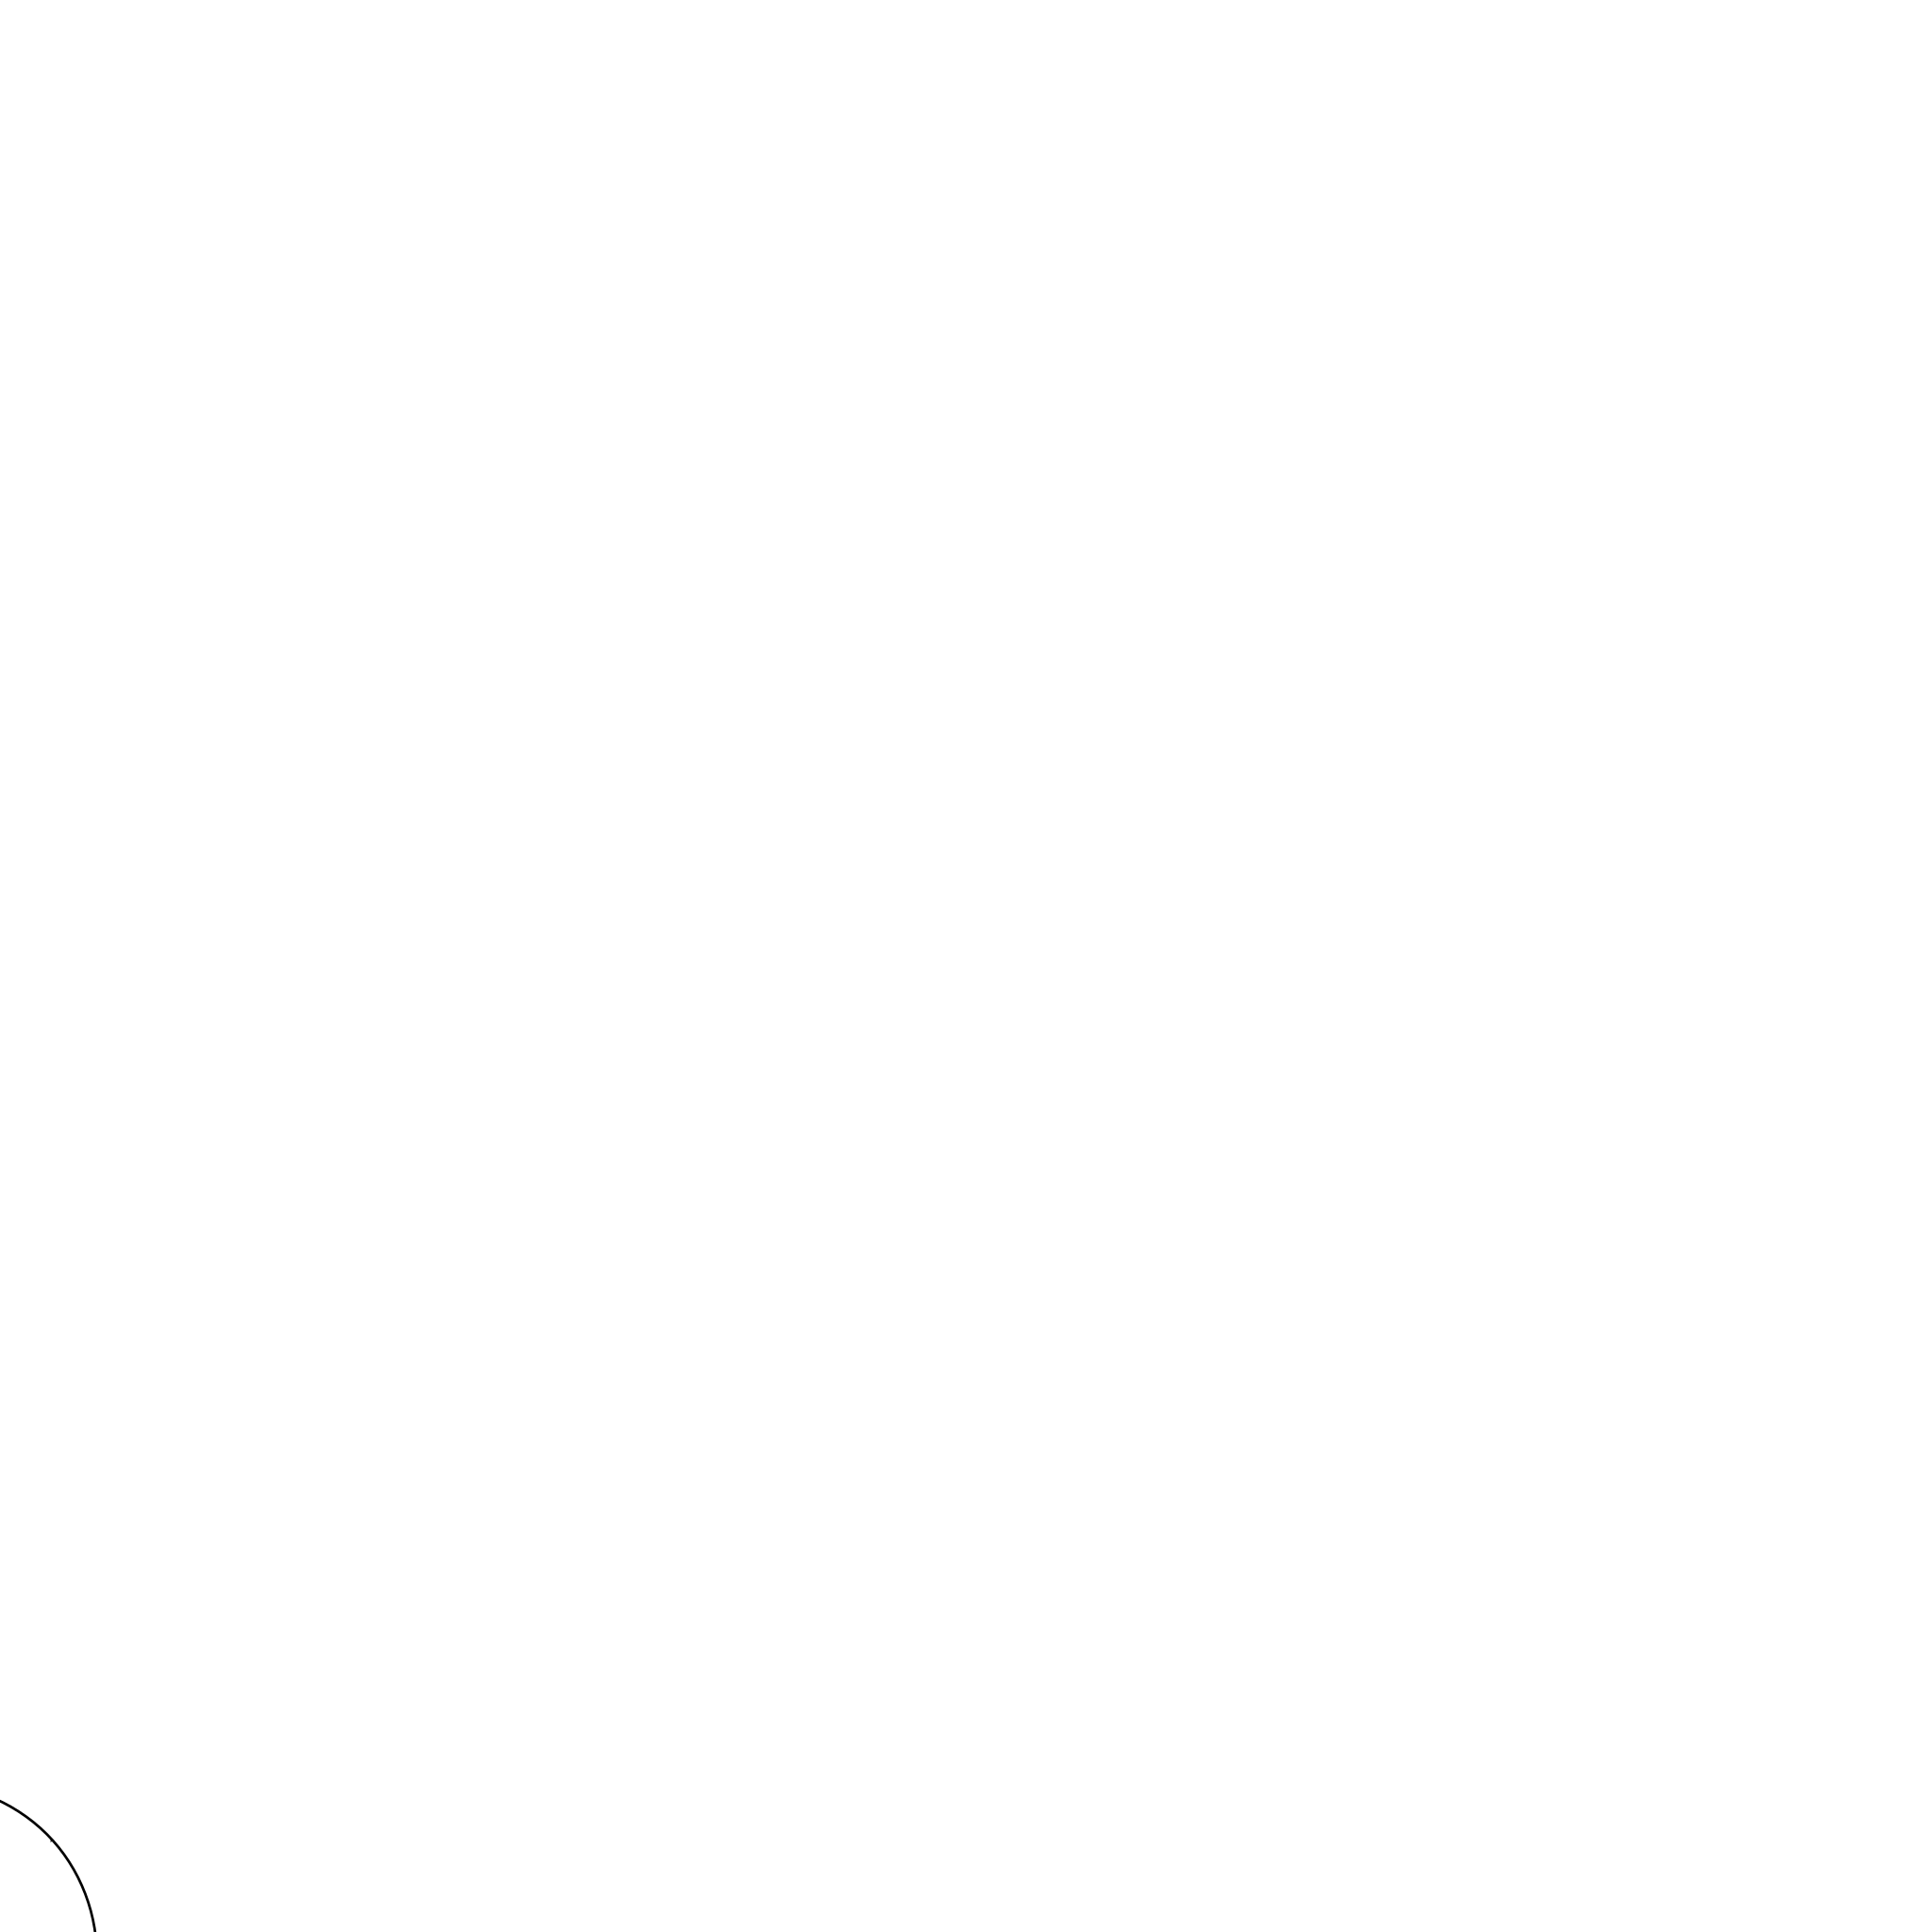
\includegraphics[width=0.4\textwidth]{w15-1}
    \label{fig:w15-1}
\end{figure}
\begin{proof}
    \[
        \left| \int\limits_{C_R} f(z)e^{iaz}dz\right| = \left| \int\limits_{0}^\pi f(Re^{i\varphi}) Rie^{i\varphi}\cdot e^{iaRe^{i\varphi}}d\varphi\right|
    .\]
Ale
\[
    e^{iaRe^{i\varphi}} = e^{iaR(\cos\varphi + i\sin\varphi)} = e^{iaR\cos\varphi} \cdot e^{-aR\sin\varphi}
.\]
Czyli
\[
    \left| \int\limits_{0}^\pi f(Re^{i\varphi})Rie^{i\varphi}\cdot e^{iaR\cos\varphi}\cdot e^{-aR\sin\varphi}d\varphi \right| \le \underset{\varphi\in[0,\pi]}{\sup}\left| f(Re^{i\varphi}) \right| R\cdot \underbrace{\int\limits_{0}^{\pi}e^{-aR\sin\varphi}d\varphi}_{J}
.\]
Stąd
\[
    J = \left| 2\int\limits_{0}^{\frac{\pi}{2}}e^{-aR\sin\varphi}d\varphi \right| \le 2\int\limits_{0}^{\frac{\pi}{2}}e^{-aR \frac{2}{\pi}\varphi}d\varphi = 2 \left.\frac{-\pi}{2aR}e^{-aR \frac{2}{\pi}\varphi}\right|_0^{\frac{\pi}{2}} = \frac{\pi}{aR}\left( 1 - e^{-aR} \right)
.\]
\[
    \int\limits_{0}^{\pi}e^{-aR\sin\varphi}d\varphi \le \underset{p\in[0,\pi]}{\sup} \left| f(Re^{i\varphi}) \right| \frac{\pi}{aR}\left( 1-e^{-aR} \right) \underset{R\to +\infty}{\longrightarrow} 0
.\]
\end{proof}
\begin{figure}[h]
    \centering
    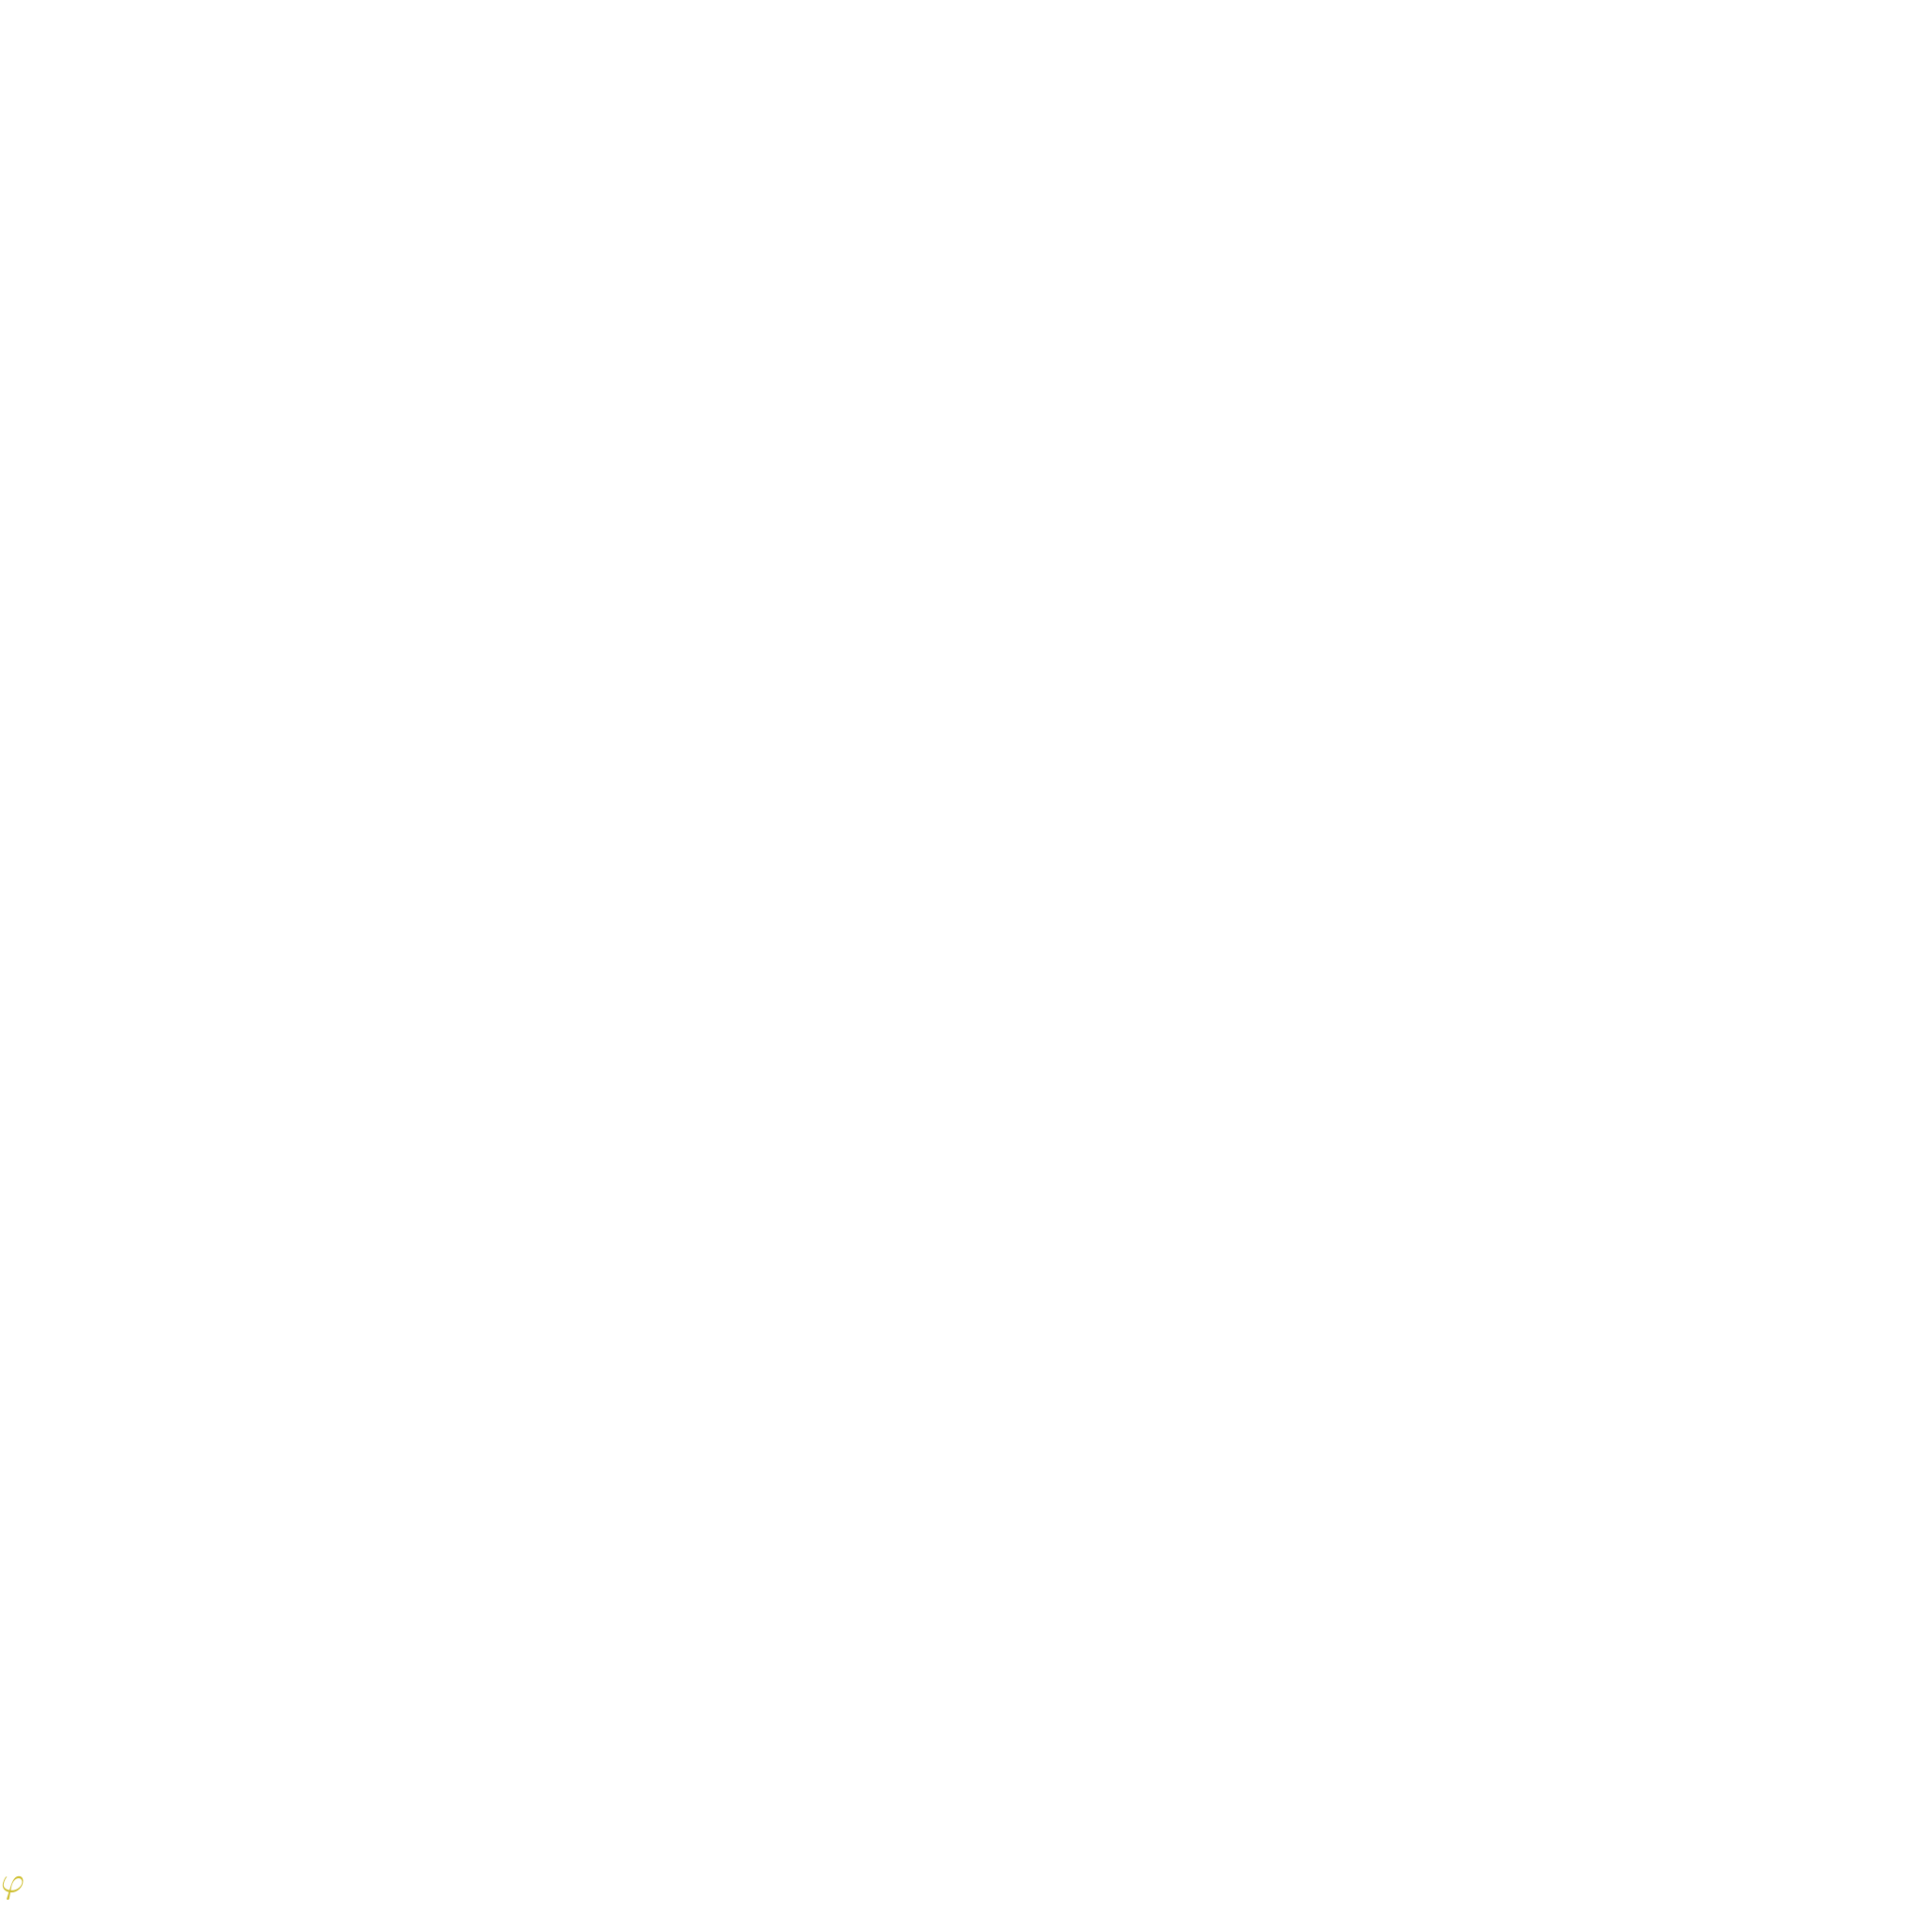
\includegraphics[width=0.3\textwidth]{w15-2}
    \caption{w15-2}
    \label{fig:w15-2}
\end{figure}

\subsection{Zachowanie funkcji wokół punktu istotnie osobliwego}
\[
    f(z) = \sum_{n=0}^{\infty} a_n(z-z_0)^n + \sum_{n=1}^{\infty} \frac{a_{-n}}{(z-z_0)^n}
.\]
\pagebreak
\begin{tw}
    (Lemat)\\
    Niech $f$ - holomorficzna i ograniczona na $R(a,0,r)$. Wówczas możemy przedłużyć $f$ do funkcji holomorficznej na $K(a,r)$. Czyli
    \[
        f(z) = c_0 + c_1(z-a)^1 + c_2(z-a)^2 + \ldots\text{, gdzie } c_0 = f(a)
    .\]
\end{tw}
\begin{proof}
    Niech
    \[H(z) = \begin{cases}
        (z-a)^2f(z)& z\neq a\\ 0 & a = a
    \end{cases}
    .\]
    Pokażemy, że $H(z)$ jest holomorficzna na $K(a,r)$. Wystarczy pokazać, że $H(z)$ jest holomorficzna w $z = a$. \\
    Policzmy $H'(a)$.
    \[
        H'(a) = \lim\limits_{h\to 0}\frac{H(a+h) - H(a)}{h} = \lim\limits_{h\to 0}\frac{(a+h-a)^2f(a+h) - 0}{h} = \lim\limits_{h\to 0}\frac{h^2f(a+h)}{h} = \lim\limits_{h\to 0} hf(a+h)
    .\]
Ale skoro $f$ - ograniczona na $R(a,0,r)$, to $0 \le \left| h f(a+h) \right| \le h M \underset{h\to 0}{\longrightarrow} 0$, czyli $H'(a) = 0$, więc $H(z)$ jest holomorficzna na $K(a,r)$.
\[
    H(z) = c_0 + c_1(z-a)^1 + c_2(z-a)^2 + \ldots
.\]
Czyli (bo $c_0 = 0$ i $c_1 = 0$, bo $H'(0) = 0$)
\[
    (z-a)^2f(z) = c_2(z-a)^2 + c_3(z-a)^3 + \ldots
.\]
Co oznacza, że nasz $f(z)$ da się przedstawić w postaci
\[
    f(z) = c_2 + c_3(z-a)^1 + \ldots
.\]
Jak położymy $c_2 \equiv f(a)$, to wtedy $f$ - holomorficzna na $K(a,r)$
\end{proof}

\begin{tw}
    (Weierstrass)\\
    Niech $f$ - holomorficzna na $R(a,0,r)$, i $a$ - punkt istotnie osobliwy funkcji $f$. Wówczas
    \[
        \underset{r>0}{\forall} \quad f(R(a,0,r)) = \mathbb{C}
    .\]
\end{tw}
\begin{proof}
    Chcemy pokazać, że $f$ - ma w $a$ punkt istotnie osobliwy i
    \[
        \underset{r > 0}{\forall} \quad \underset{c\in \mathbb{C}}{\forall} \quad \underset{\varepsilon > 0}{\forall} \quad \underset{z}{\exists} \quad \left| z-a \right| < r \implies \left| f(z) - c \right| < \varepsilon
    .\]
Przez sprzeczność.\\
Wiemy, że $f$ ma w $a$ punkt istotnie osobliwy oraz
\[
    \underset{r > 0}{\exists} \quad \underset{c\in\mathbb{C}}{\exists} \quad \underset{\varepsilon > 0}{\exists} \quad \underset{z}{\forall} \left| z-a \right| < r , \left| f(z) - c \right| \ge \varepsilon
.\]
Pokażemy, że wyżej wymienione zdanie jest sprzeczne z tym, że $f$ ma w $a$ punkt istotnie osobliwy.\\
Jeżeli
\[
    \underset{z}{\forall} \left| z - a \right| < r, \left| f(z) - c \right| \ge \varepsilon
,\]
to znaczy, że funkcja $g(z) = \frac{1}{f(z) - c}$ jest ograniczona i holomorficzna na $R(a,0,r)$. Oznacza to, że możemy przedłużyć $g(z)$ do funkcji holomorficznej na $K(a,r)$. Czyli możemy rozwinąć $z$ w szereg Laurenta na $K(a,r)$.
\[
    g(z) = a_0 + a_1(z-a) + a_2(z-a)^2 + \ldots
.\]
\begin{enumerate}[i)]
    \item Jeżeli $a_0 \neq 0$, to znaczy, że $g(a) \neq 0$, czyli
         \[
             0 \neq a_0 = \frac{1}{f(a) - c}
        ,\]
    to znaczy, że $f(a) - c = \frac{1}{a_0} \implies f(a) = c+ \frac{1}{a_0}$ i sprzecznośc, bo jeżeli $f$ ma w $a$ konkretną wartość a na $R(a,0,r)$ jest holomorficzna to wtedy możemy zapisać
        \[
            f(z) = c + \frac{1}{a_0} + b_1(z-z_0) + b_2(z-z_0)^2 + \ldots
        ,\]
    a skoro $f$ ma w $a$ punkt istotnie osobliwy, to jej rozwinięcie powinno wyglądać tak:
        \[
            f(z) = \sum_{k = 0}^{\infty} d_k(z-a)^k + \sum_{k = 1}^{\infty} \frac{e_k}{(z-a)^k}
        .\]
    Jeżeli $a_0 = a_1 = a_2 = \ldots = a_n =  0$, to znaczy, że
        \[
            g(z) = (z-a)^n\left( c_0 + \underbrace{c_1(z-a) + c_2(z-a)^2 + \ldots }_{g_1(z)}\right)
        .\]
    Zauważmy, że $g_1(z)$ jest holomorficzna i $g_1(a) \neq 0$, możemy więc rozwinąć $\frac{1}{g_1(z)}$ w $K(a,r)$
        \[
            \frac{1}{g_1(z)} = f_0 + f_1(z-a) + f_2(z-a)^2 + \ldots
        .\]
\end{enumerate}

\end{proof}

\end{document}
